\section{Resultados}

\subsection{Sobre la climatología del tamaño de los CTs}
\begin{frame}
\begin{itemize}
    \item Se analizaron {\red 191} y {\gray 337} CTs de las cuencas {\red NA} y {\gray EP} respectivamente durante el período 2000-2020.
    \\~\
    \item Sólo se consideran las posiciones de CT de 6 horas que se localizan en la región de estudio. Se obtuvieron {\red 4526} y {\gray 6923} posiciones de CTs para las cuencas.
\end{itemize}
\end{frame}

\begin{frame}
    \begin{figure}
        \centering
        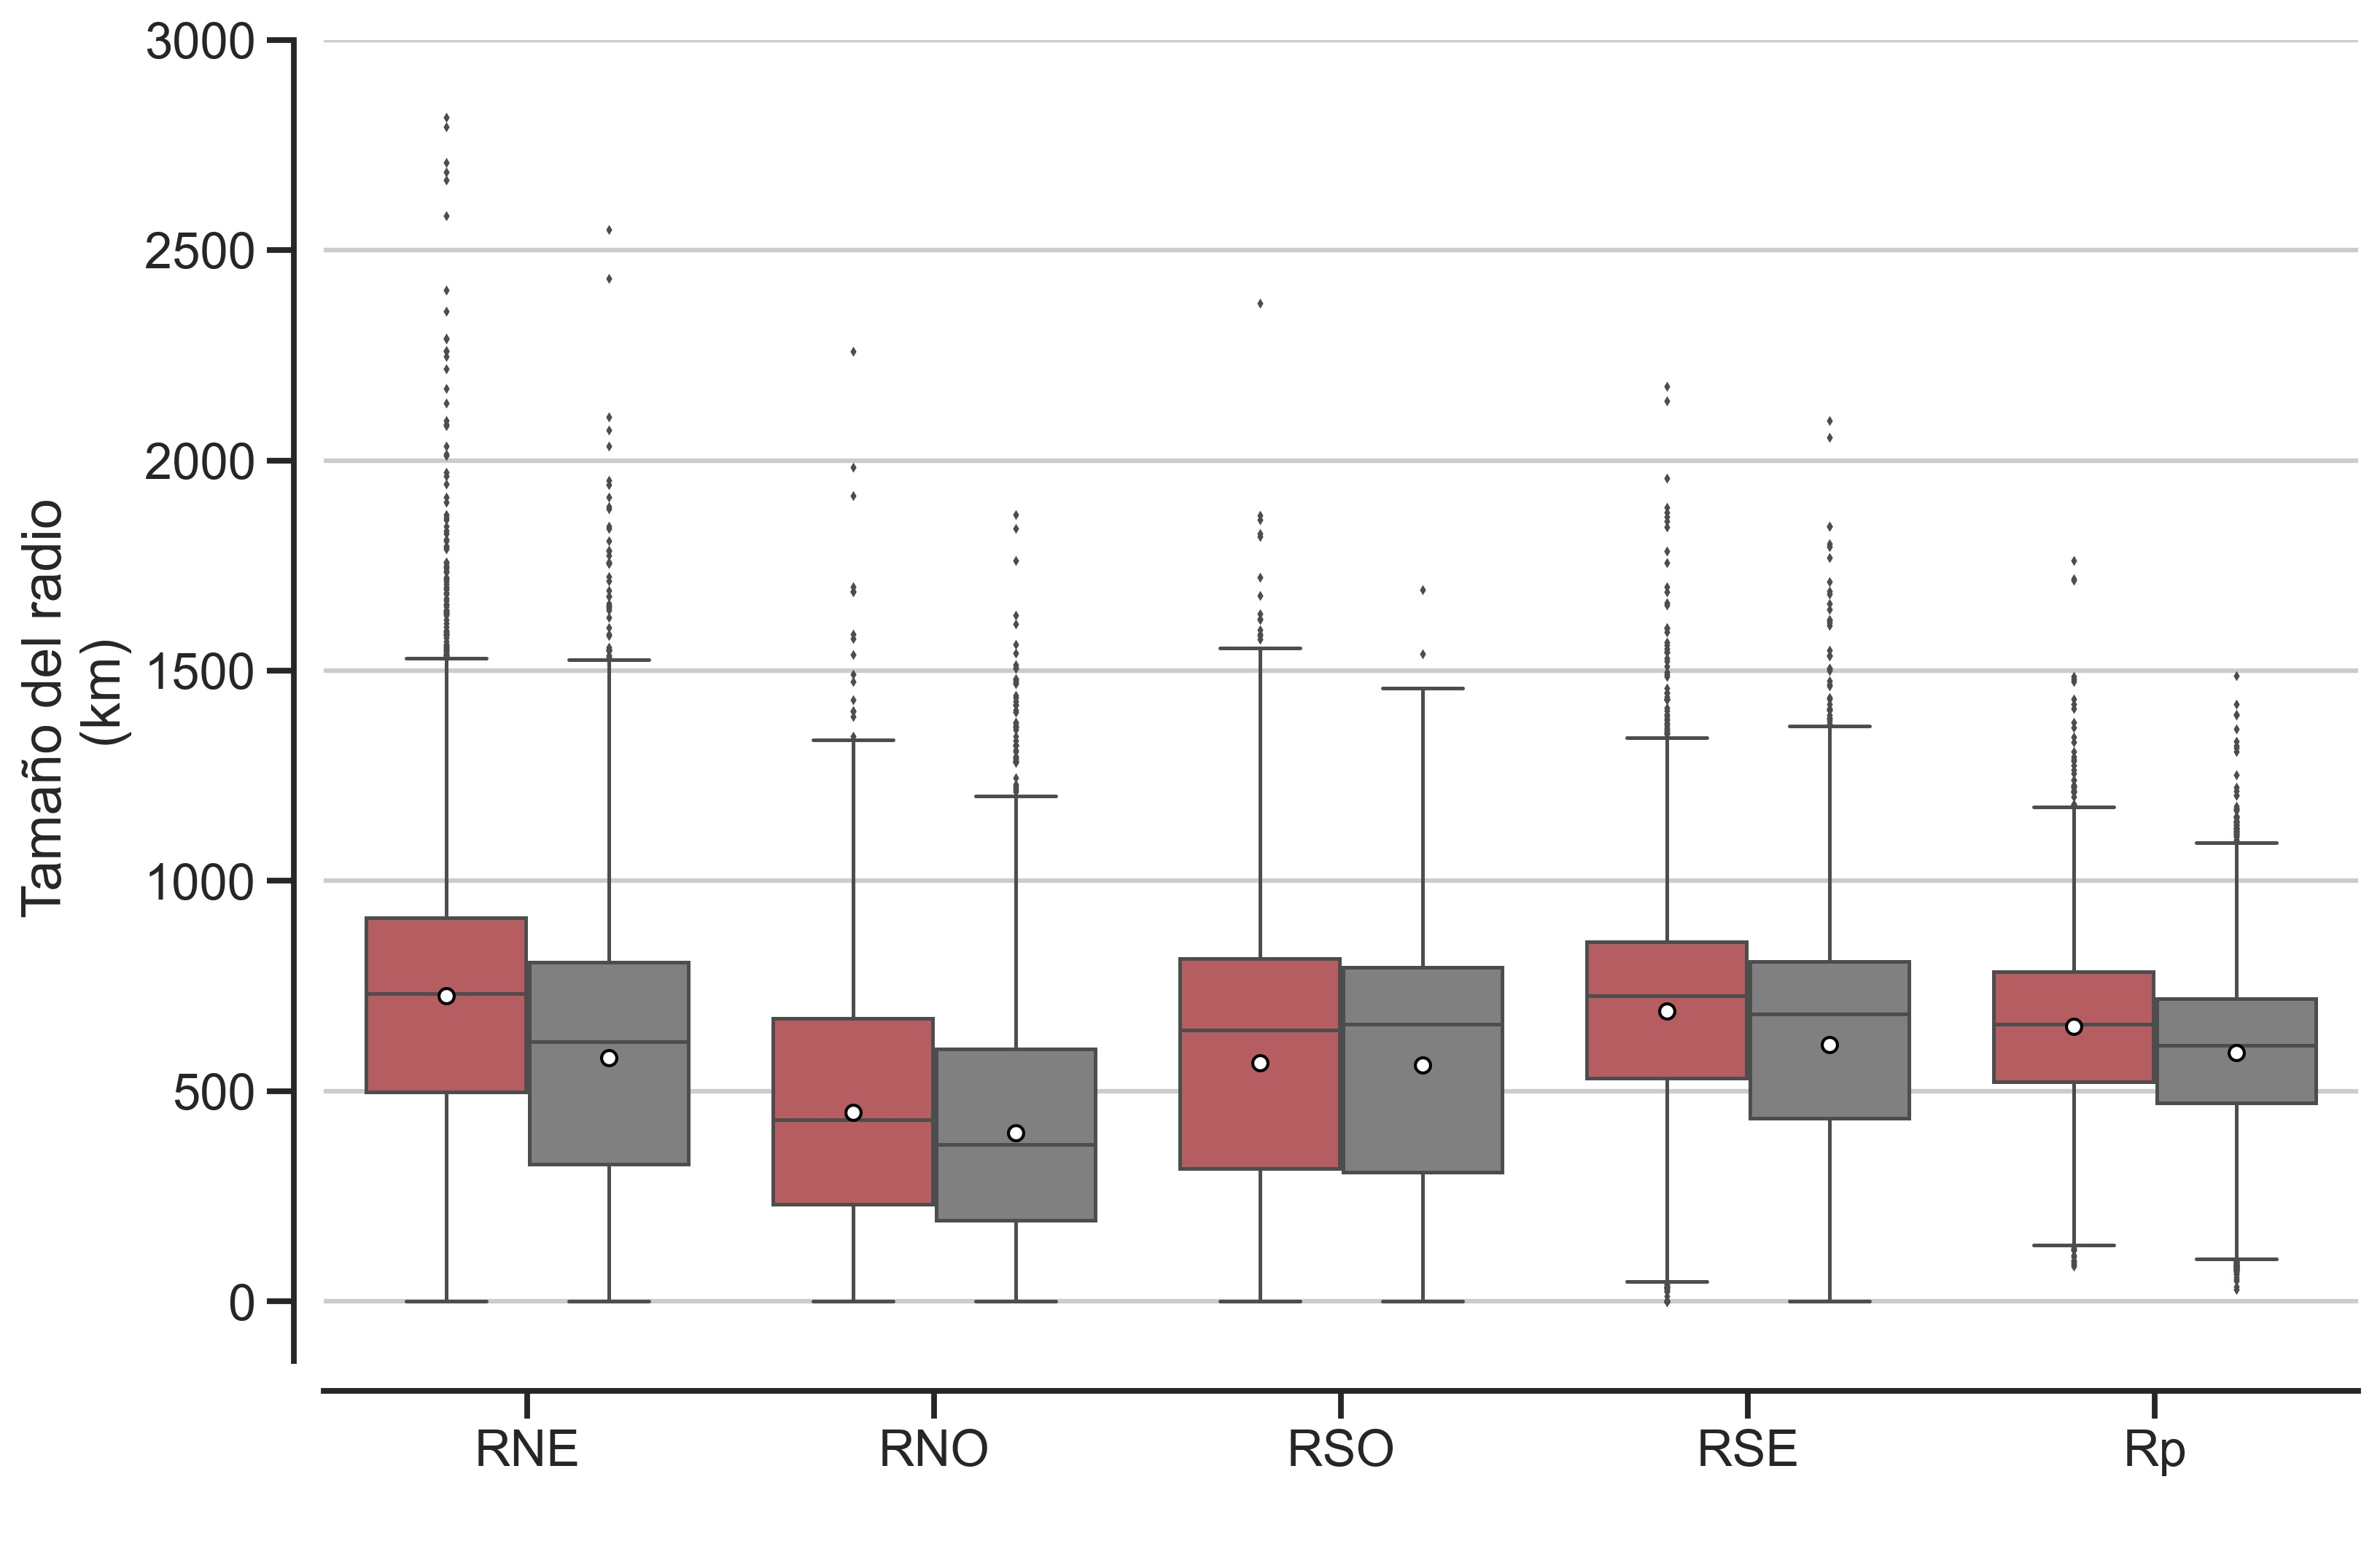
\includegraphics[scale = 0.35]{Images/Figures/Fig_3_1.jpeg}
        \caption{Cajas y bigotes de las distribuciones de los radios por cuadrante y el $R_p$ (km) de los radios en la región de estudio de la cuenca {\red NA} y {\gray EP}.}
        \label{fig:fig_9}
    \end{figure}
\end{frame}

\begin{frame}
    \begin{columns}
        \begin{column}{0.4\textwidth}
            \begin{enumerate}
                \setcounter{enumi}{0}
                \item Sobre la variación espacial de los tamaños
            \begin{block}{Figura 9:}
                Distribución espacial del tamaño de los CTs por cuadrante (km): (a) RNE, (b) RNO, (c) RSO, (d) RSE y (e) $R_p$. Los límites en la barra de colores representan los rangos intercuantílicos (p25 y p75) durante el período 2000-2020.
            \end{block}
            \end{enumerate}
        \end{column}
        \begin{column}{0.6\textwidth}
        \begin{figure}
            \centering
            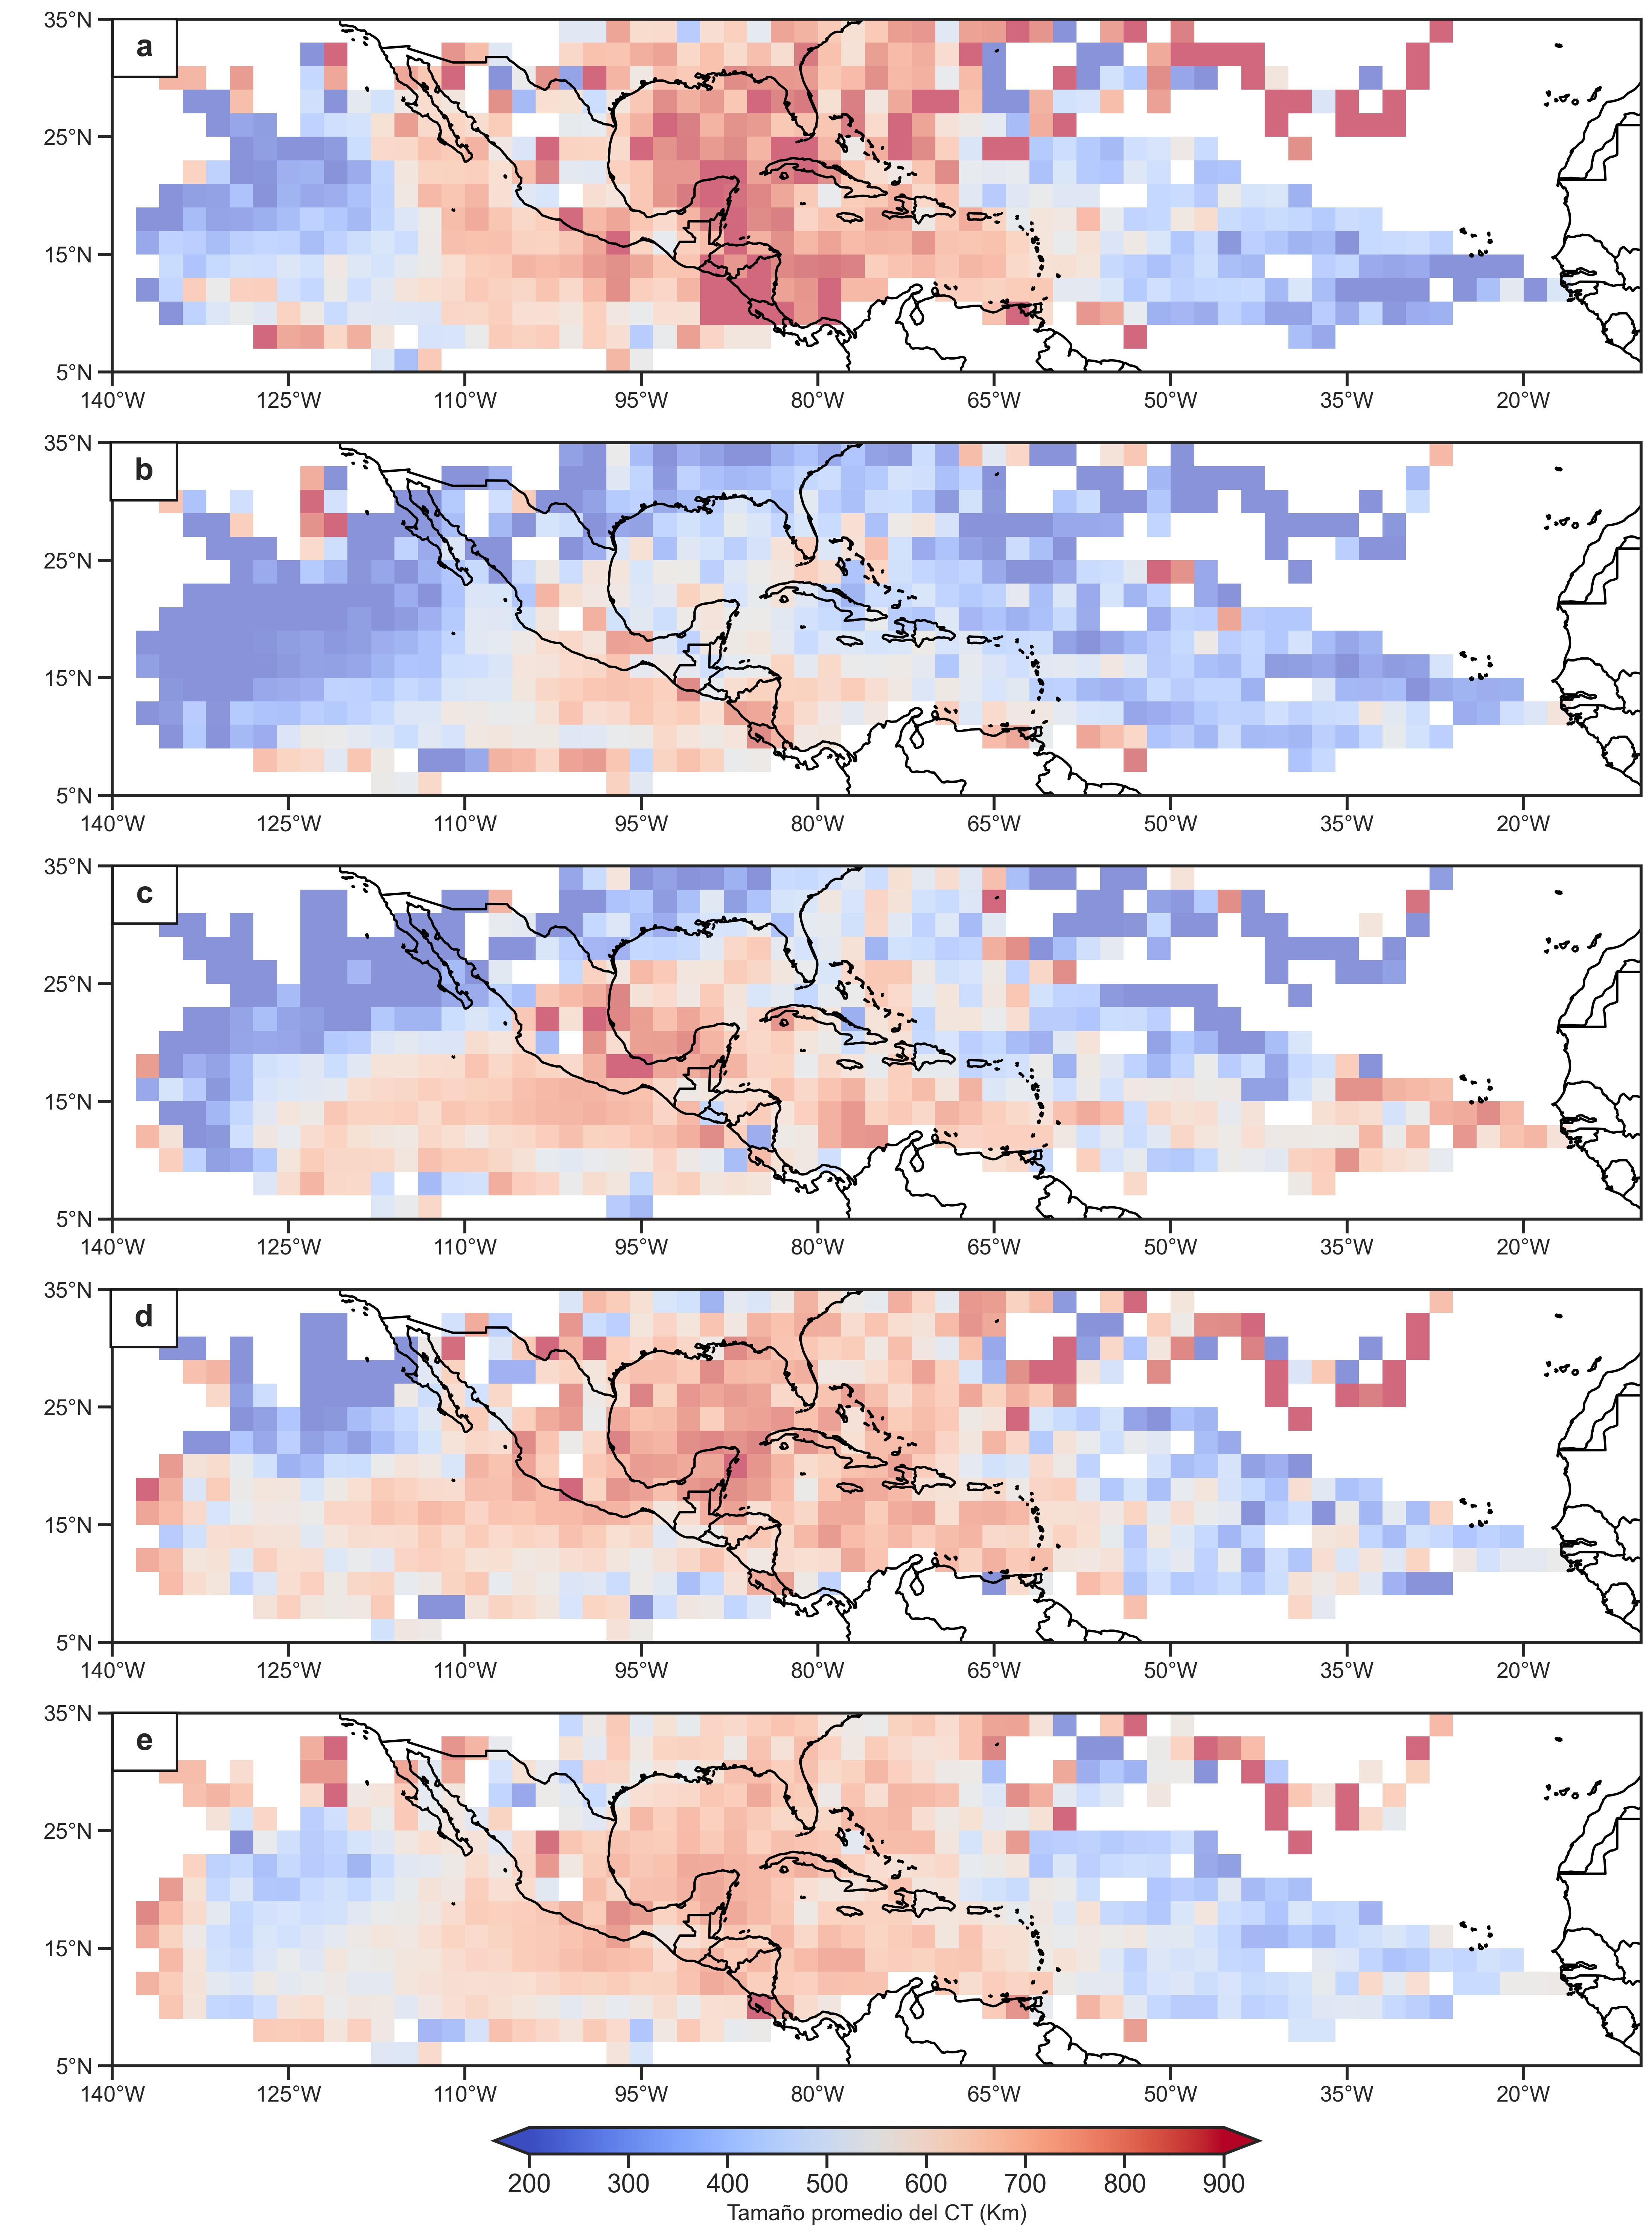
\includegraphics[scale = 0.17]{Images/Figures/Fig_3_6.jpeg}
            \caption{}
            \label{fig:fig_tamaño}
        \end{figure}
        \end{column}
    \end{columns}
\end{frame}

\begin{frame}
    \begin{enumerate}
    \setcounter{enumi}{0}
    \item Sobre la variación espacial de los tamaños
    \begin{figure}
        \centering
        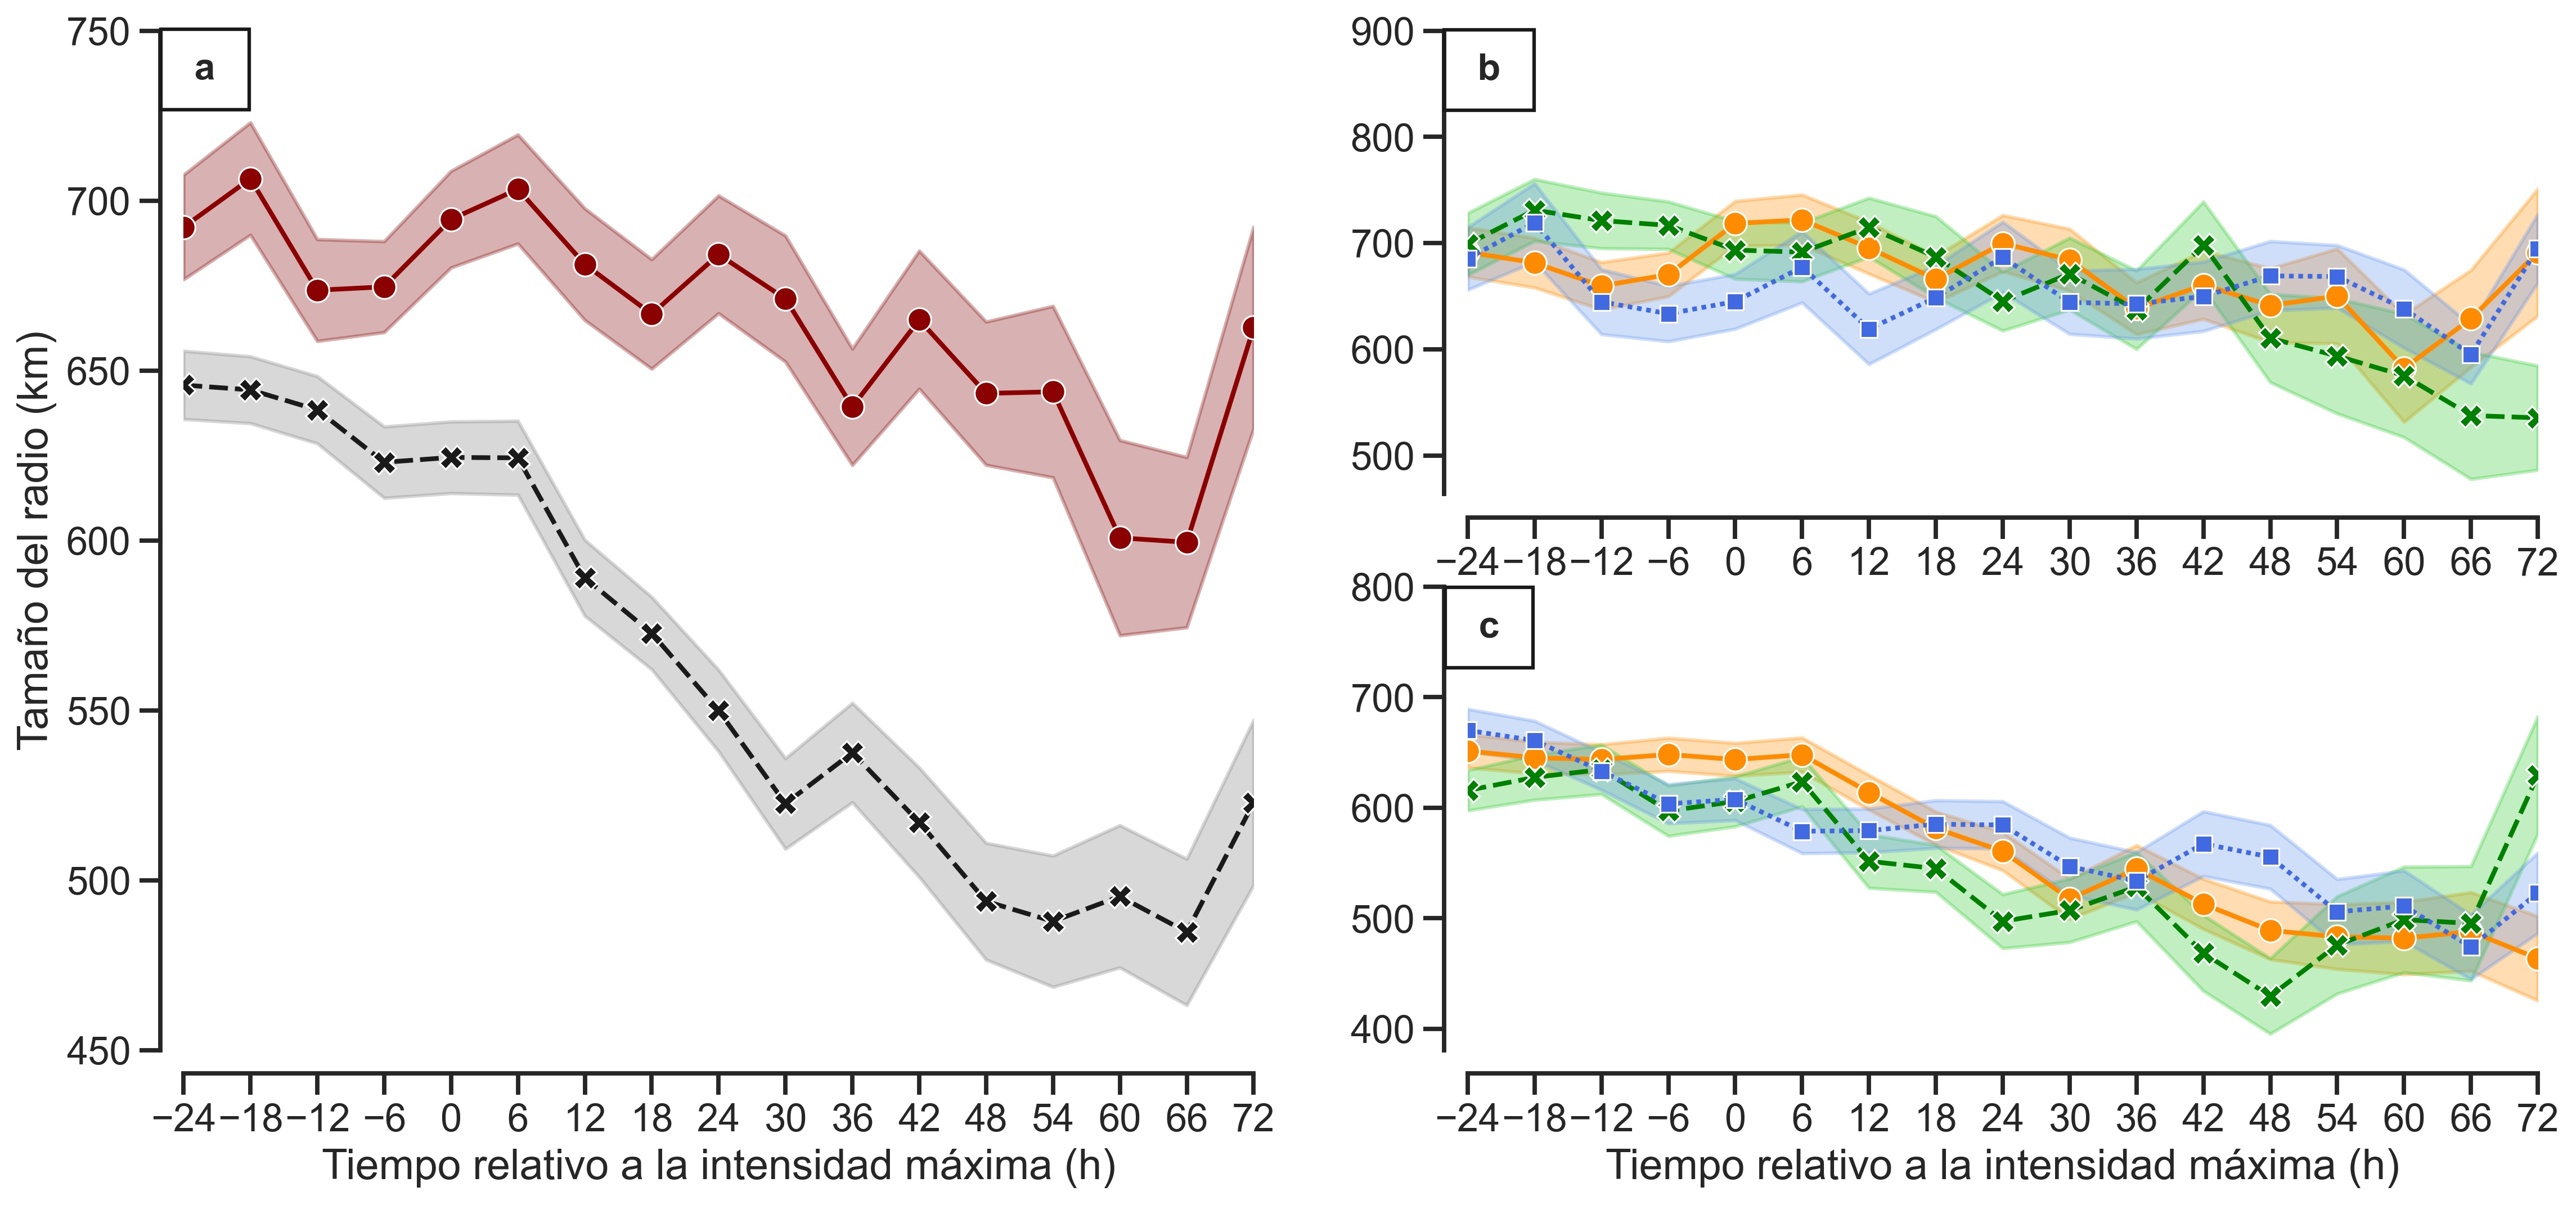
\includegraphics[scale = 0.26]{Images/Figures/Fig_3_8.jpeg}
        \caption{Compuestos de tamaño de Rp (km) de: (a) los CTs sobre {\red NA} y {\gray EP} y las TTs (en amarillo), HUR1-2 (en verde) y HUR3-5 (en azul) sobre (b) {\red NA} y (c) {\gray EP}. El tiempo 0 h representa el momento en que alcanzan la máxima intensidad. Las áreas sombreadas proporcionan el error estándar asociado al valor promedio de $R_p$ cada 6 h.}
        \label{fig:fig_11}
    \end{figure}
    \end{enumerate}
\end{frame}

\begin{frame}
    \begin{enumerate}
    \setcounter{enumi}{1}
        \item Sobre la variación mensual de los tamaños
    \end{enumerate}
    \begin{figure}
        \centering
        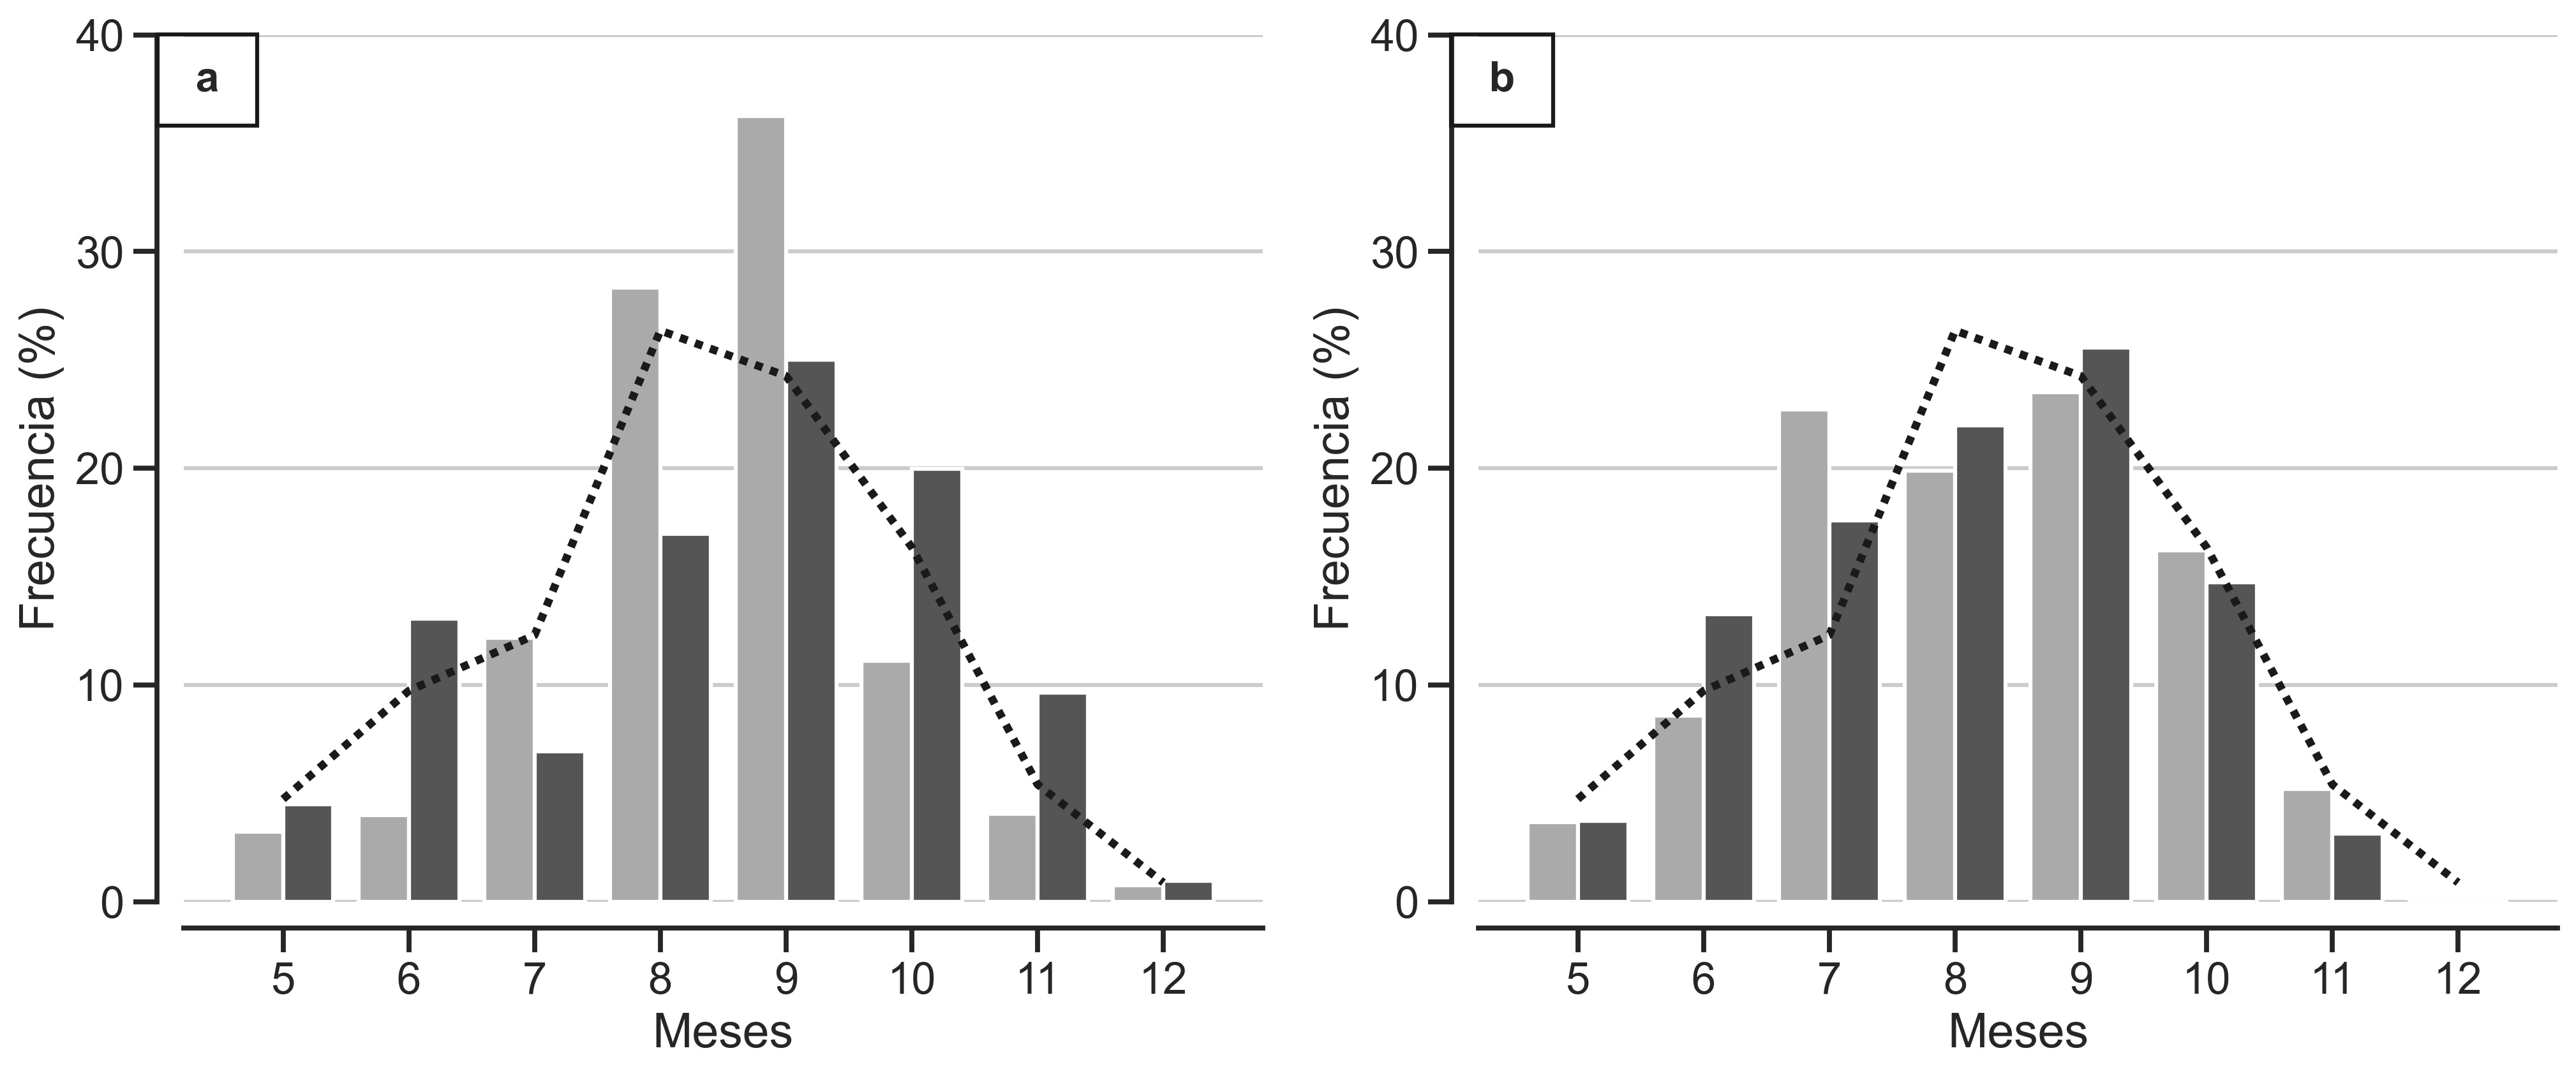
\includegraphics[scale = 0.3]{Images/Figures/Fig_3_10.jpeg}
        \caption{Tamaños mensuales de CT para los cuartiles inferior (pequeño) y superior (grande) en: (a) cuencas {\red NA} y (b) {\gray EP}.}
        \label{fig:fig_12}
    \end{figure}
\end{frame}

\subsection{Sobre la relación del tamaño y la precipitación}
\begin{frame}
\begin{enumerate}
\setcounter{enumi}{0}
    \item Climatología de los tamaños usando productos IMERG
\end{enumerate}
    \begin{figure}
        \centering
        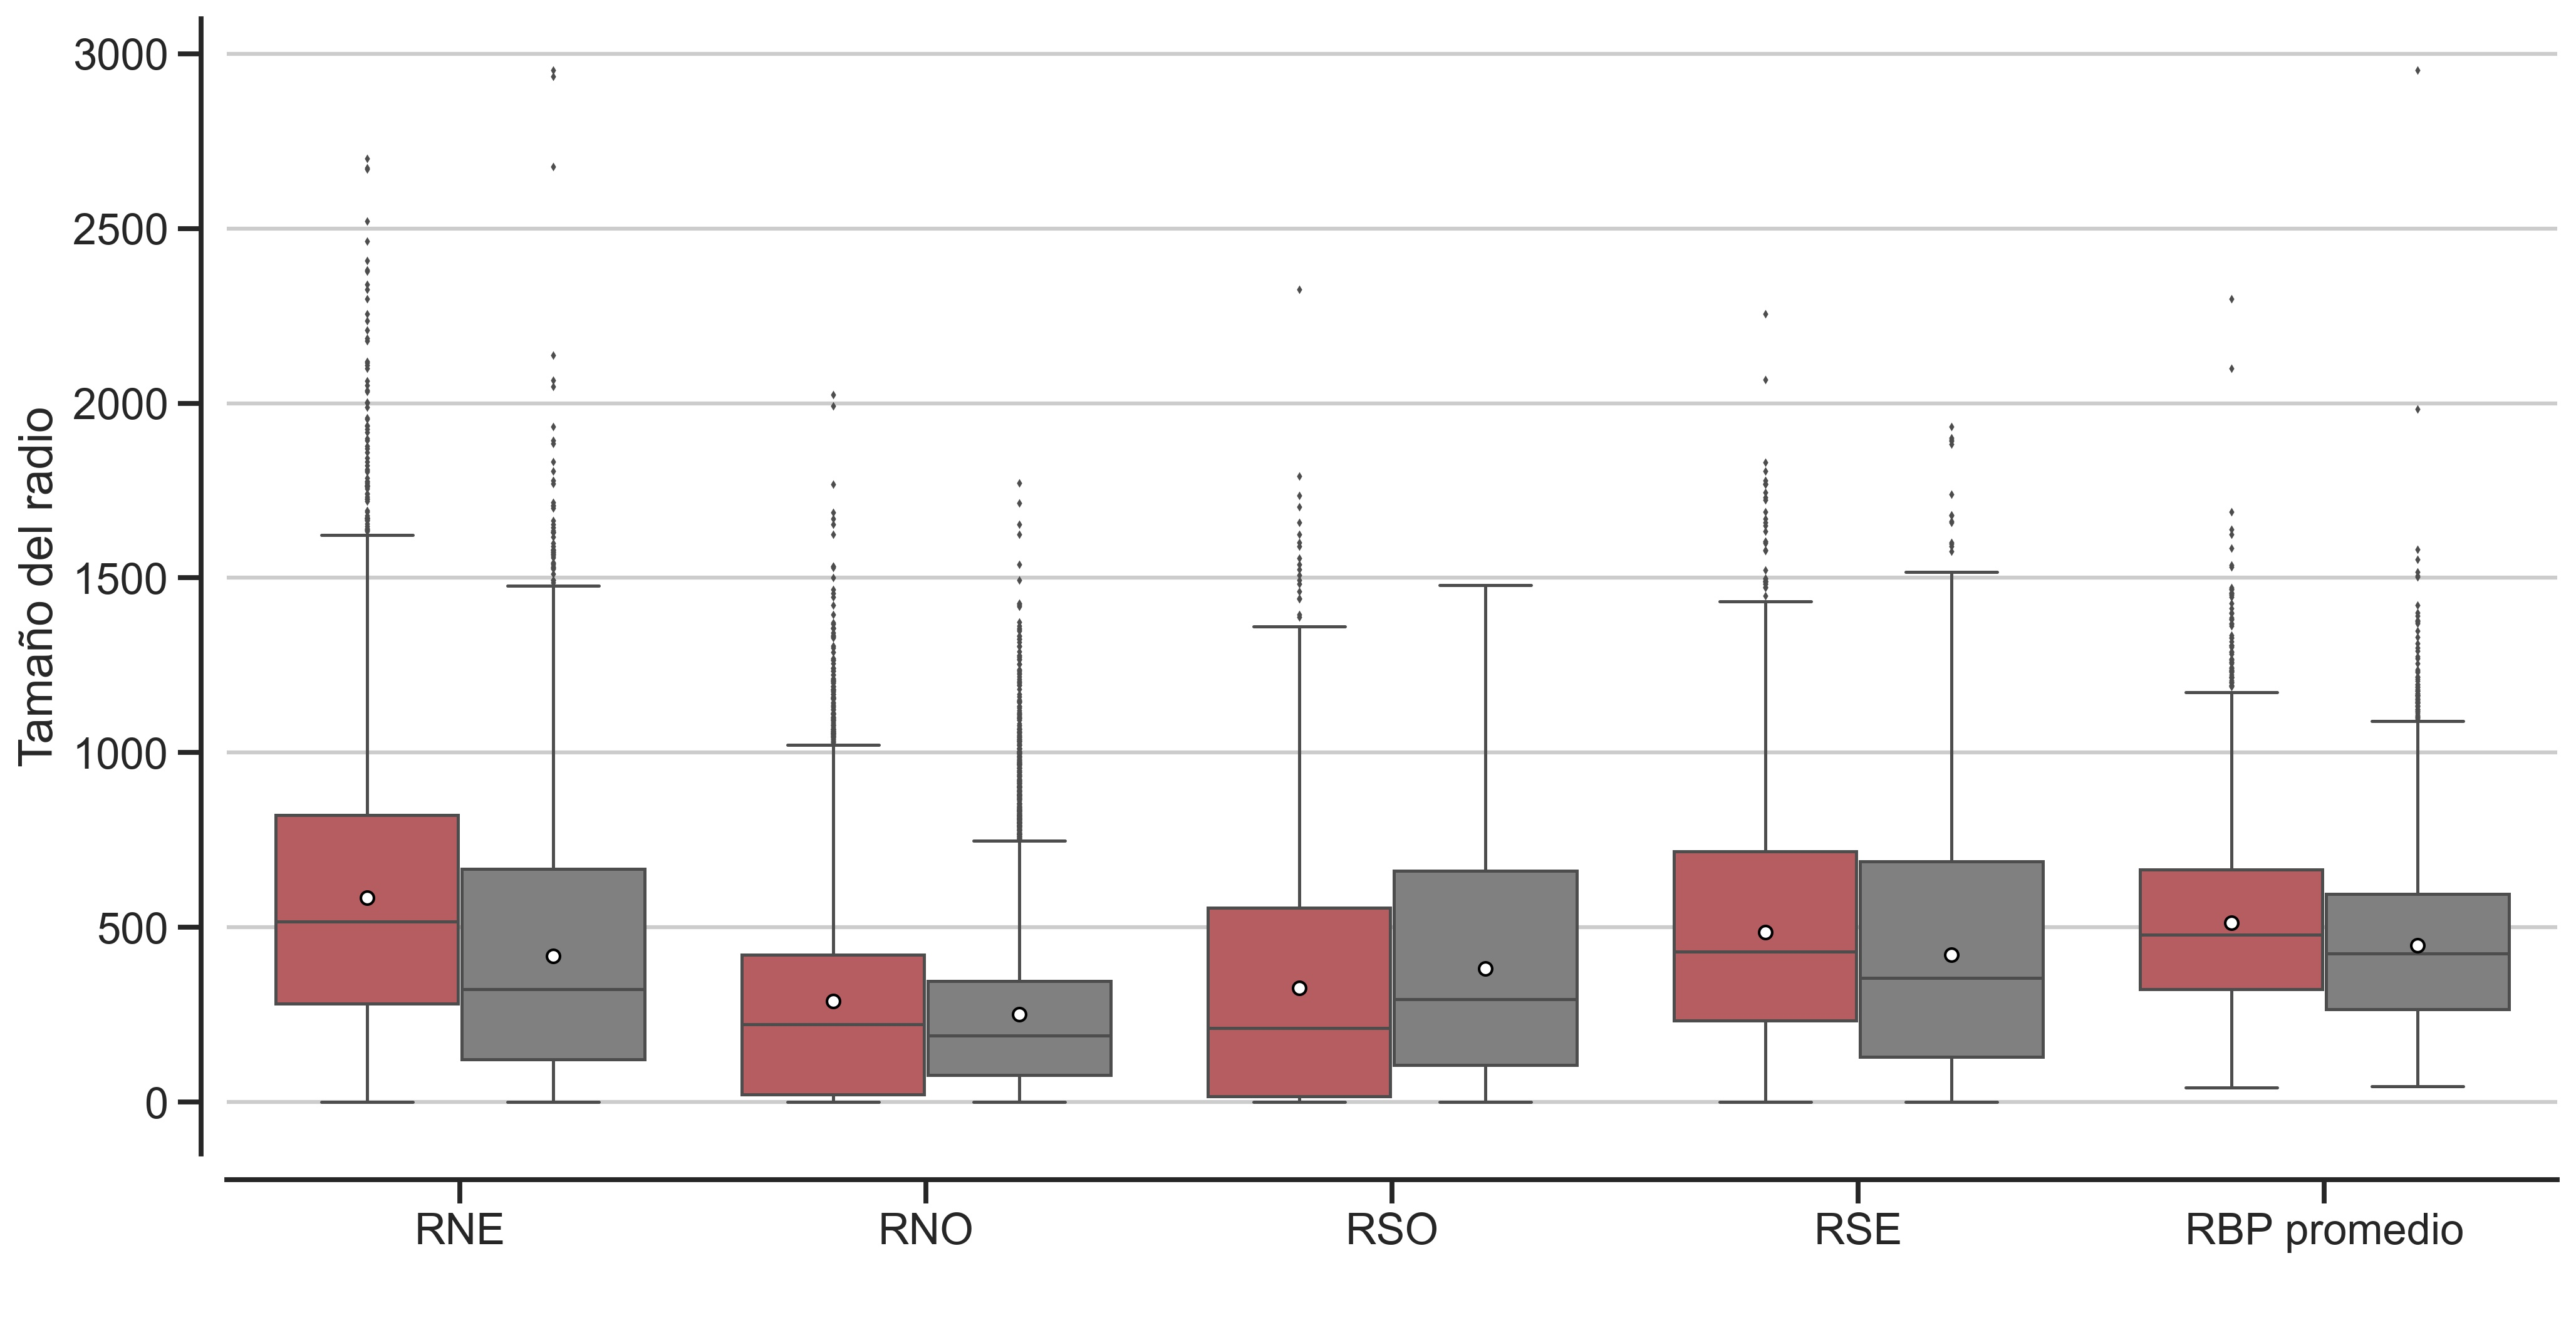
\includegraphics[scale = 0.3]{Images/Figures/Fig_3_13.jpeg}
        \caption{Cajas y bigotes de las distribuciones de los radios por cuadrante y el $R_p$ (km) de los radios en la región de estudio de la cuenca {\red NA} y {\gray EP} definidos por el algoritmo RBP.}
        \label{fig:fig_13}
    \end{figure}
\end{frame}

\begin{frame}
    \begin{exampleblock}{Para el NA}
        % Please add the following required packages to your document preamble:
% \usepackage{booktabs}
% \usepackage{graphicx}
\begin{table}[H]
\centering
\caption{Correlación de rango de Spearman (r) entre los tamaños calculados con las técnicas de ROCLOUD y RBP para cada cuadrante y promedio; Se determinan para la cuenca NA. Los valores con un asterisco son significativos a un nivel del 95\% de confianza.}
\label{tab:3.5}
\resizebox{\textwidth}{!}{%
\begin{tabular}{@{}llllll@{}}
\toprule
             & RNE\_RPB       & RNO\_RPB       & RSO\_RPB       & RSE\_RPB       & Rp\_RPB        \\ \midrule
RNE\_ROCLOUD & \textit{0.81*} &                &                &                &                \\
RNO\_ROCLOUD & \textit{0.14}  & \textit{0.67*} &                &                &                \\
RSO\_ROCLOUD & \textit{0.05}  & \textit{0.17}  & \textit{0.63*} &                &                \\
RSE\_ROCLOUD & \textit{0.32*} & \textit{0.09}  & \textit{0.18}  & \textit{0.66*} &                \\
Rp\_ROCLOUD  & \textit{0.59*} & \textit{0.32*} & \textit{0.37*} & \textit{0.5*}  & \textit{0.73*} \\ \bottomrule
\end{tabular}%
}
\end{table}
    \end{exampleblock}
\end{frame}

\begin{frame}
    \begin{alertblock}{Para el EP}
        % Please add the following required packages to your document preamble:
% \usepackage{booktabs}
% \usepackage{graphicx}
\begin{table}[H]
\centering
\caption{Igual a la Cuadro \ref{tab:3.5}, pero para el EP}
\label{tab:3.6}
\resizebox{\textwidth}{!}{%
\begin{tabular}{@{}llllll@{}}
\toprule
             & RNE\_RPB       & RNO\_RPB       & RSO\_RPB       & RSE\_RPB       & Rp\_RPB        \\ \midrule
RNE\_ROCLOUD & \textit{0.77*} &                &                &                &                \\
RNO\_ROCLOUD & \textit{0.32*} & \textit{0.71*} &                &                &                \\
RSO\_ROCLOUD & \textit{0.12}  & \textit{0.21}  & \textit{0.69*} &                &                \\
RSE\_ROCLOUD & \textit{0.26}  & \textit{0.08}  & \textit{0.28}  & \textit{0.67*} &                \\
Rp\_ROCLOUD  & \textit{0.56*} & \textit{0.38*} & \textit{0.48*} & \textit{0.57*} & \textit{0.74*} \\ \bottomrule
\end{tabular}%
}
\end{table}
    \end{alertblock}
\end{frame}

\begin{frame}
\begin{enumerate}
\setcounter{enumi}{1}
    \item Dependencia de la PCT con el tamaño del CT: GPM\_MERGIR
\end{enumerate}
    \begin{columns}
        \begin{column}{0.6\textwidth}
        \begin{figure}
            \centering
            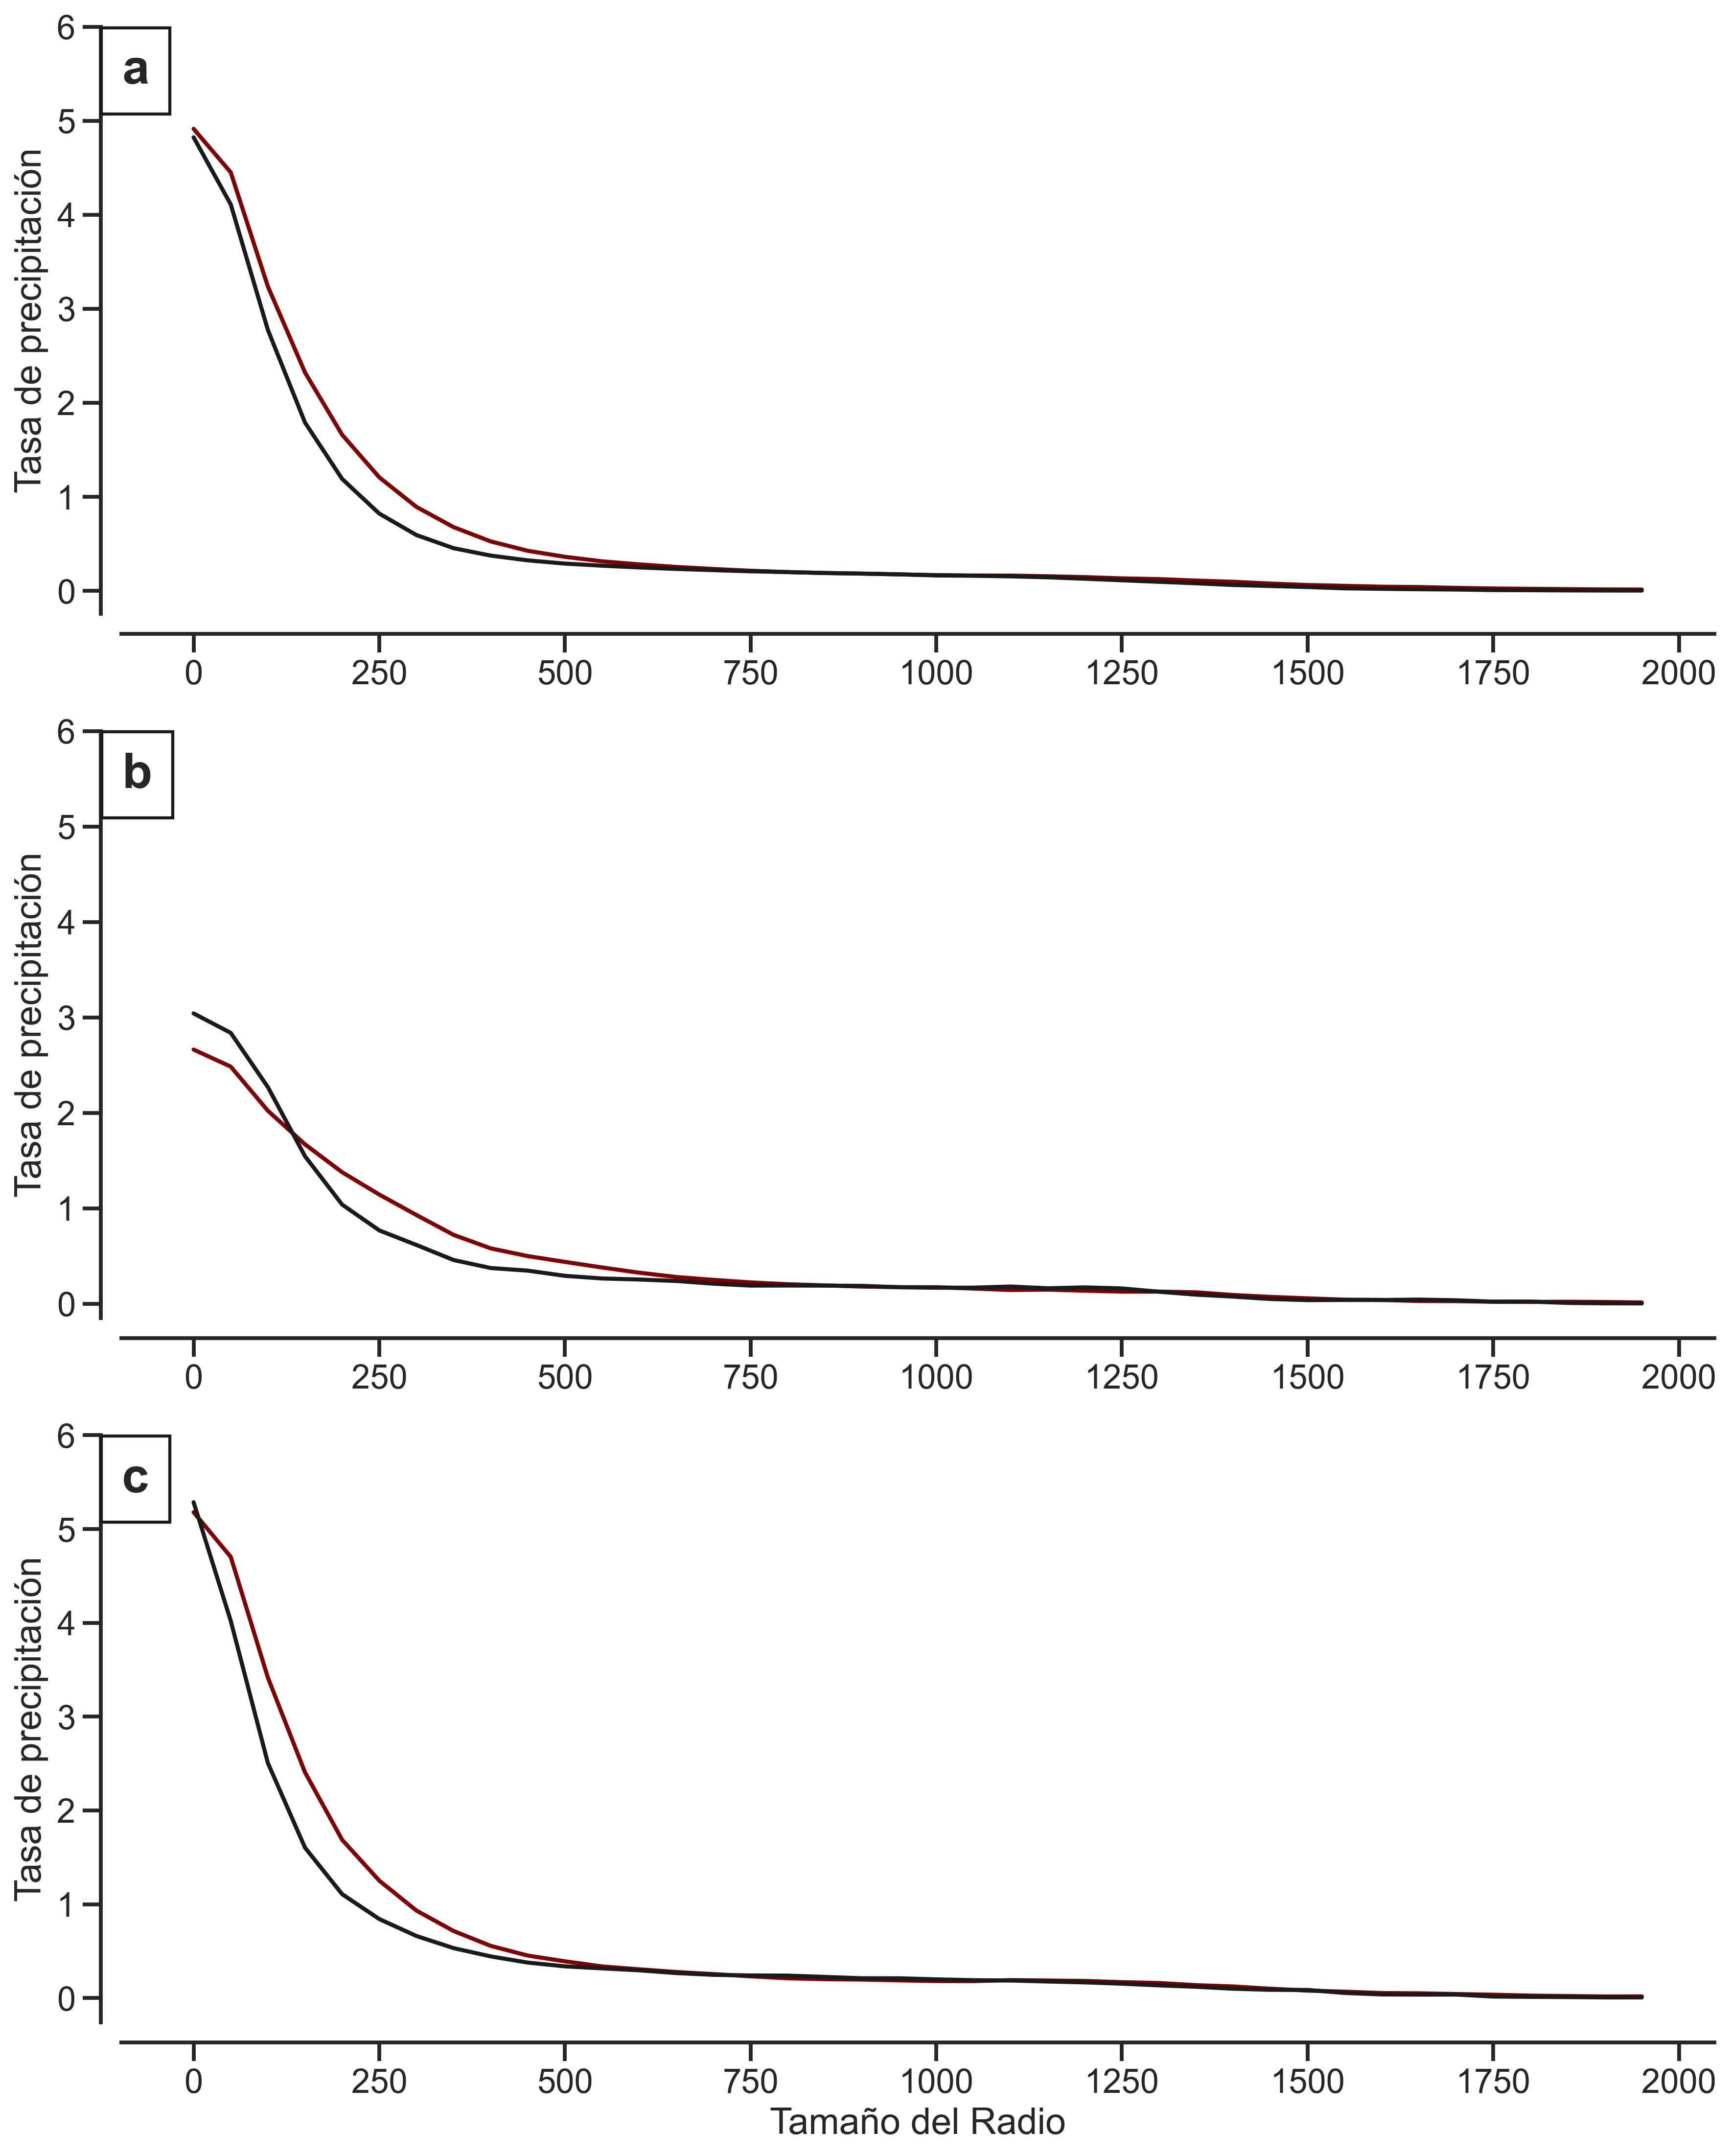
\includegraphics[scale = 0.215]{Images/Figures/Fig_3_16.jpeg}
            \caption{}
            \label{fig:fig_rbp}
        \end{figure}
        \end{column}
        
        \begin{column}{0.4\textwidth}
            \begin{block}{Figura 13:}
                Tasa de precipitación ($mm h^{-1}$) de IMERG del CT en función del radio (km), medido por la técnica de anillos, para (a) todas las posiciones, (b) posiciones sobre continente y (c) posiciones que se encuentren al menos a 250 km de la costa.
            \end{block}
        \end{column}
    \end{columns}
\end{frame}

\begin{frame}
\begin{enumerate}
\setcounter{enumi}{2}
    \item Dependencia de la PCT con el tamaño del CT: CHIRPS
\end{enumerate}
    \begin{figure}
        \centering
        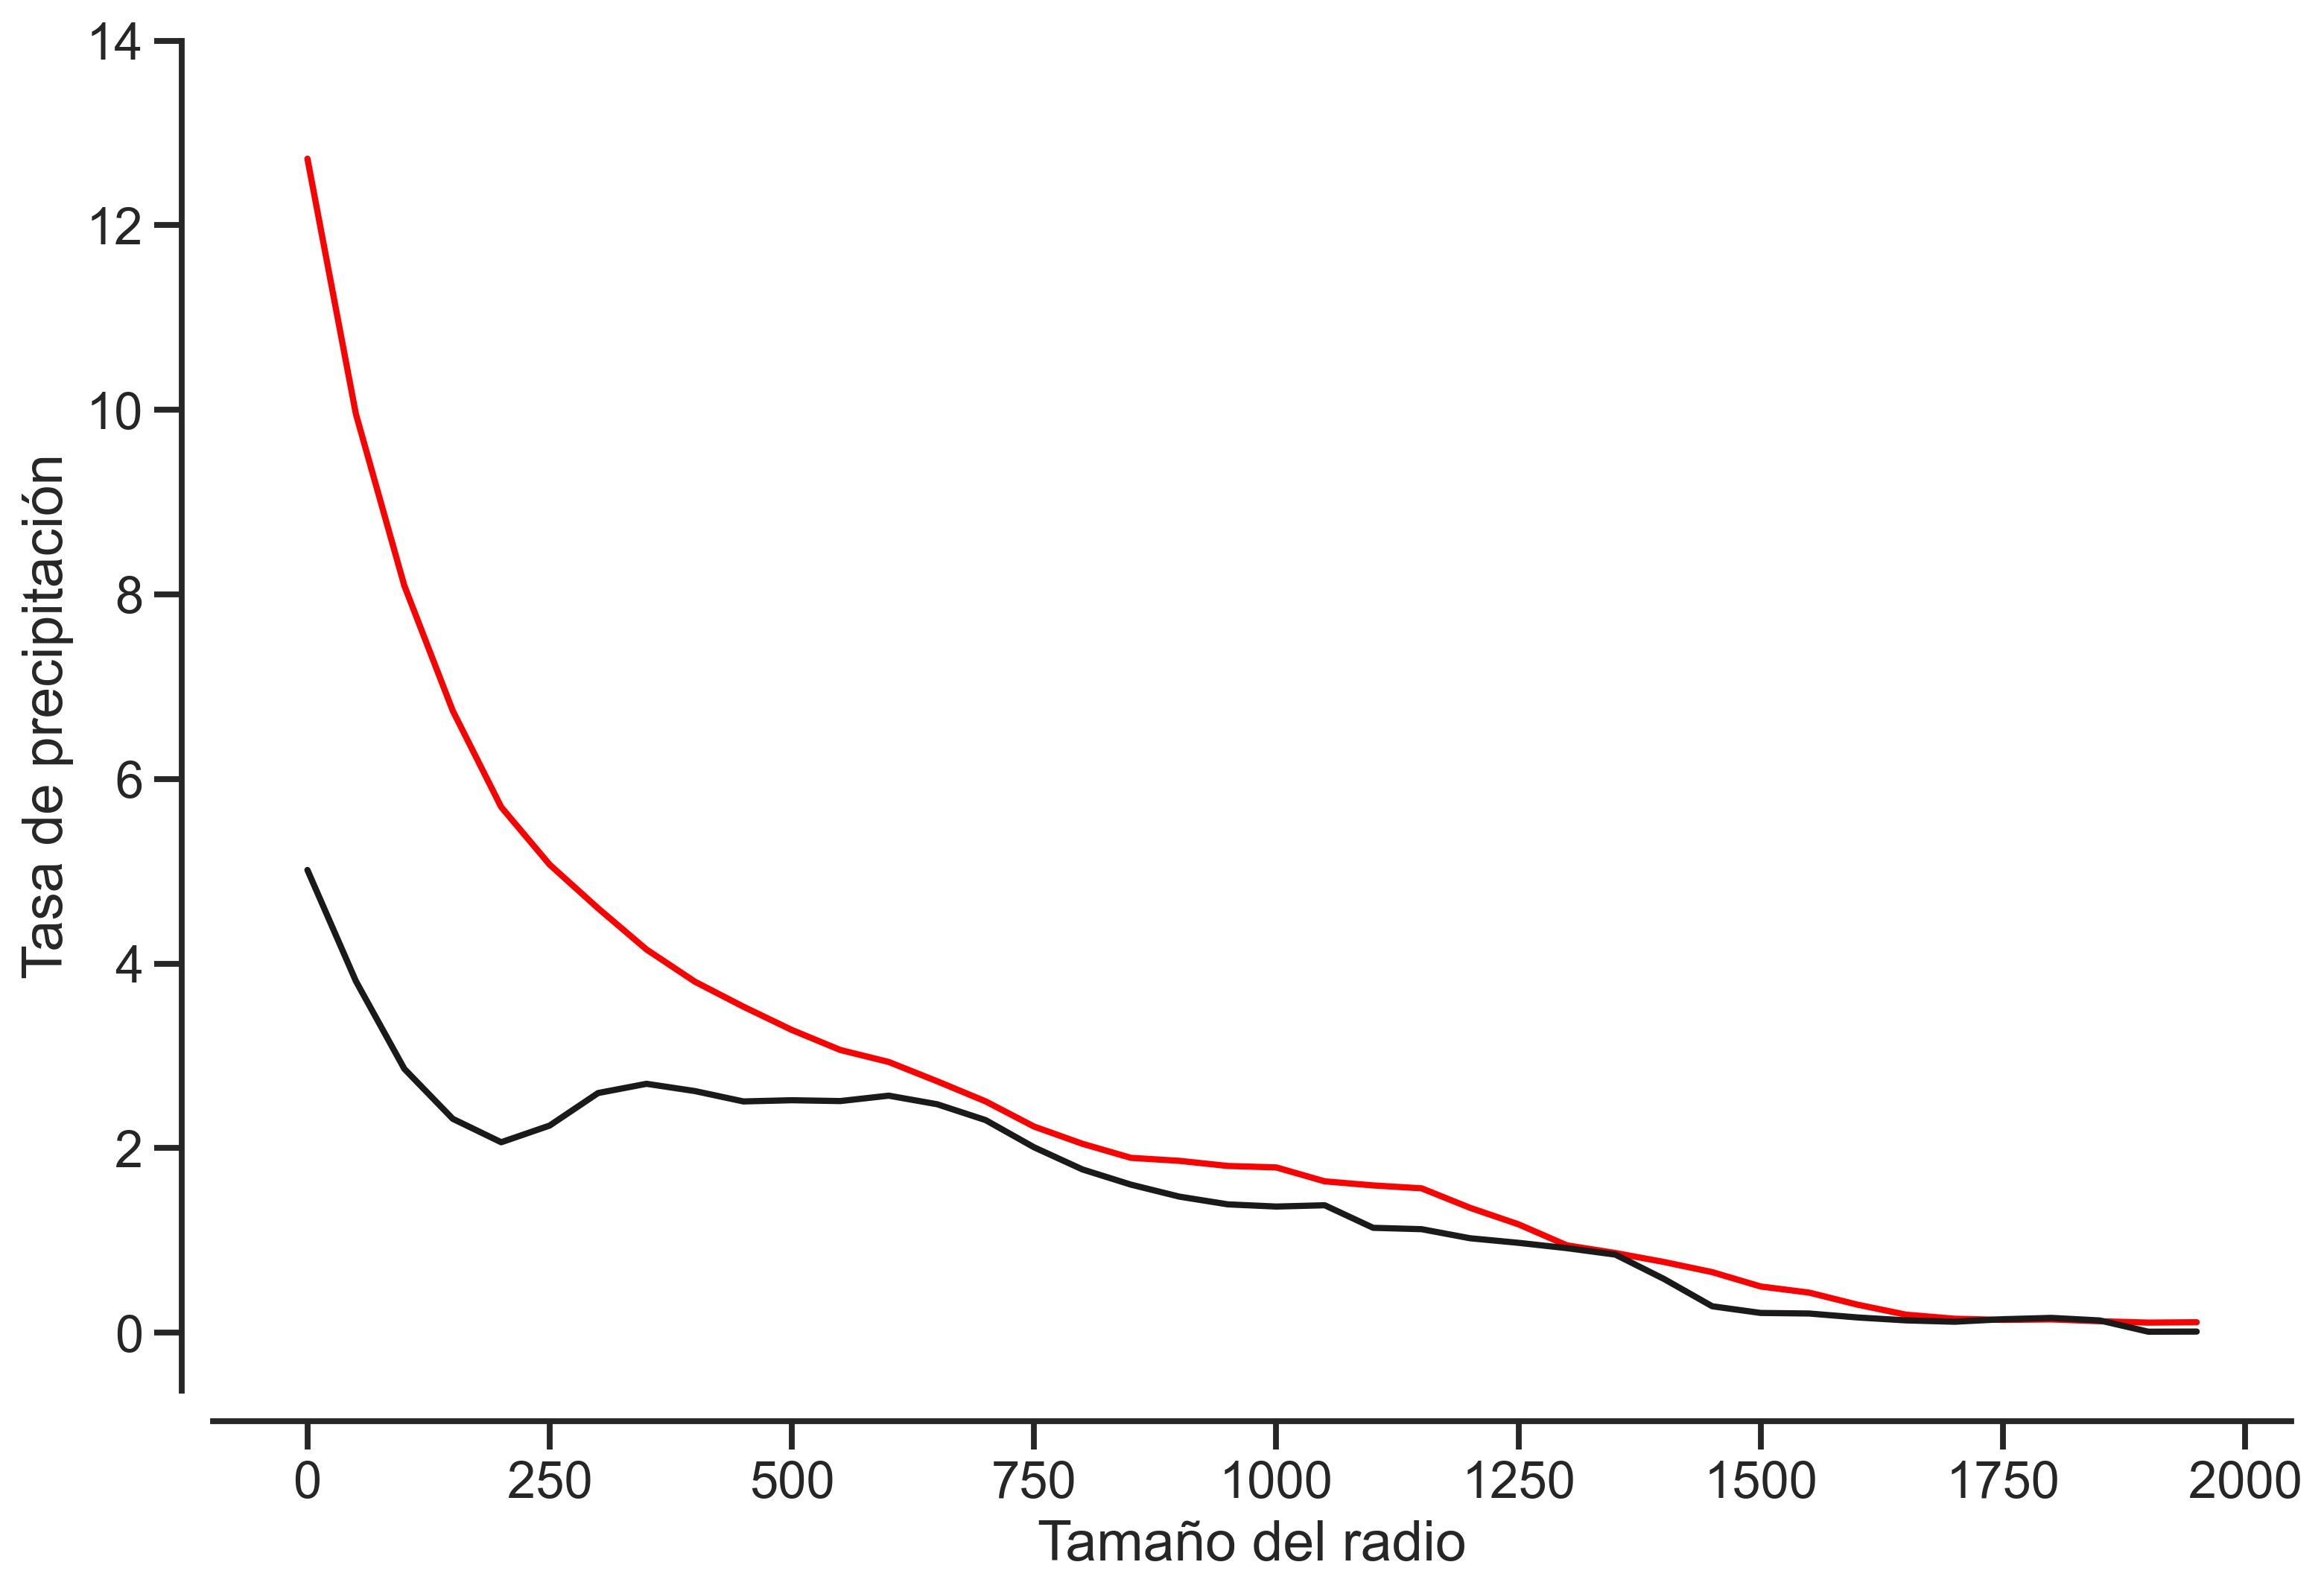
\includegraphics[scale = 0.35]{Images/Figures/Fig_3_21.jpeg}
        \caption{Tasa de precipitación (mm $h^{-1}$) del CTs en función de su tamaño (km), definido por los rangos intercuartílicos del tamaño definido por ROCLOUD, en las cuencas: (a) {\red NA} y (b) {\gray EP}.}
        \label{fig:figchirps}
    \end{figure}
\end{frame}

\subsection{Sobre las variables medioambientales y la precipitación}
\begin{frame}
% Please add the following required packages to your document preamble:
% \usepackage{booktabs}
% \usepackage{graphicx}
% \usepackage[table,xcdraw]{xcolor}
% If you use beamer only pass "xcolor=table" option, i.e. \documentclass[xcolor=table]{beamer}
\begin{table}[H]
\centering
\caption{Coeficientes y estimación de modelos de la lluvia acumulada diaria en el área del CT para la cuenca NA y EP. Unidad de PCP: $10^{3}$ mm.}
\label{tab:3.8}
\resizebox{\textwidth}{!}{%
\begin{tabular}{@{}ccc@{}}
\toprule

{\color[HTML]{000000} \textit{\textbf{Variables}}} & {\color[HTML]{000000} \textit{\textbf{Coeficientes del modelo NA}}} & {\color[HTML]{000000} \textit{\textbf{Coeficientes del modelo EP}}} \\ \midrule
 
{\color[HTML]{000000} Intersección con el eje}     & {\color[HTML]{000000} 13.66}                                        & {\color[HTML]{000000} -17.45}                                       \\

{\color[HTML]{000000} $V_{max}$}                        & {\color[HTML]{000000} 0.01}                                        & {\color[HTML]{000000} 0.02}                                        \\
 
{\color[HTML]{000000} $R_p$}                          & {\color[HTML]{000000} 0.23}                                        & {\color[HTML]{000000} 0.22}                                        \\

{\color[HTML]{000000} \textit{PNM}}                         & {\color[HTML]{000000} -0.02}                                        & {\color[HTML]{000000} -0.02}                                       \\
 
{\color[HTML]{000000} \textit{HE}}                          & {\color[HTML]{000000} 21.14}                                        & {\color[HTML]{000000} 20.89}                                        \\

{\color[HTML]{000000} \textit{CIZ}}                         & {\color[HTML]{000000} 0.42}                                        & {\color[HTML]{000000} 0.20}                                        \\

{\color[HTML]{000000} \textit{DIV}}                         & {\color[HTML]{000000} 180.4}                                        & {\color[HTML]{000000} 186.4}                                       \\

{\color[HTML]{000000} Número de casos}             & {\color[HTML]{000000} 4526}                                         & {\color[HTML]{000000} 6993}                                         \\
{\color[HTML]{000000} RMSE}                        & {\color[HTML]{000000} 0.529}                                        & {\color[HTML]{000000} 0.498}                                        \\
{\color[HTML]{000000} QIC}                         & {\color[HTML]{000000} 453}                                          & {\color[HTML]{000000} 699}                                          \\ \bottomrule
\end{tabular}%
}
\end{table}
\end{frame}

\subsection{Sobre la forma del CT}
\begin{frame}
\begin{figure}
    \centering
    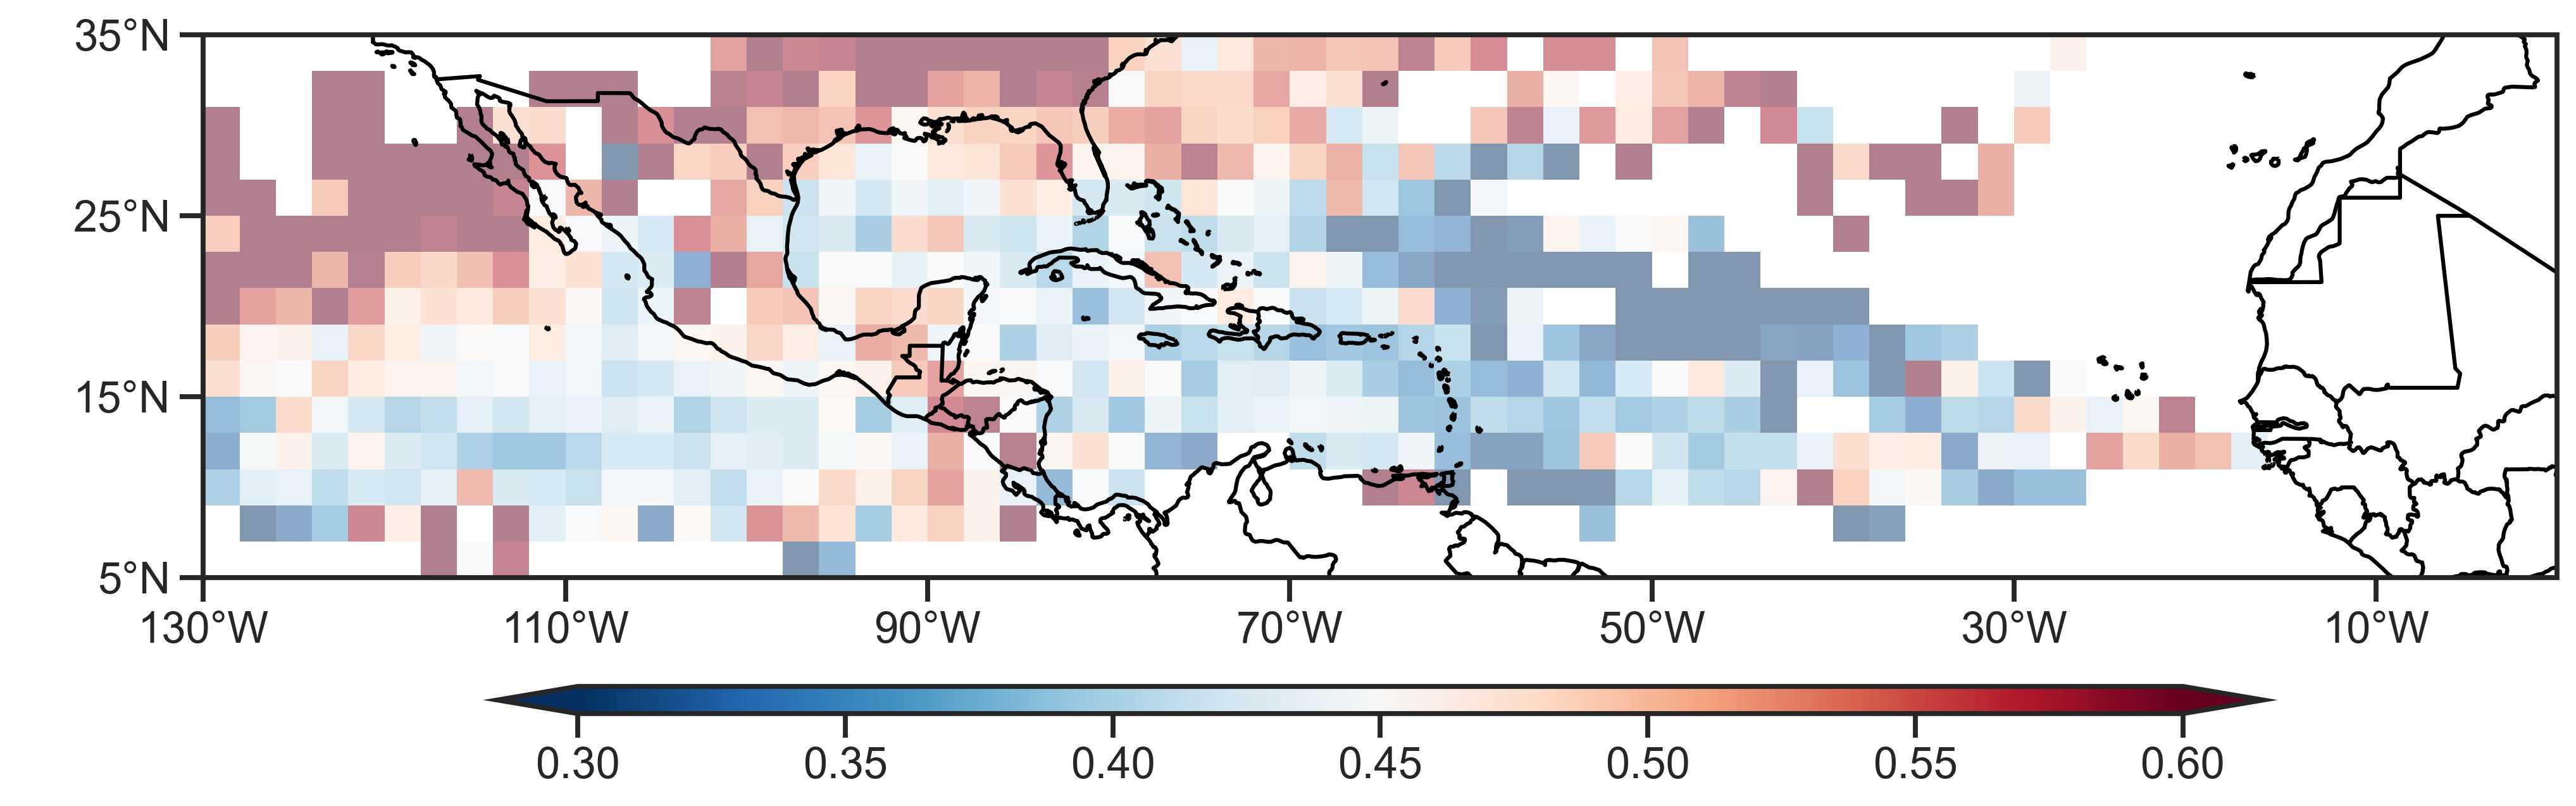
\includegraphics[scale = 0.3]{Images/Figures/Fig_3_26_1.jpeg}
    \caption{Distribución espacial en una malla de 2 $\times$ 2°de la métrica de $D$ de los CTs analizados. Los rangos de color en la escala fueron determinados por los rangos intercuartílicos}
    \label{fig:fig_10}
\end{figure}
\end{frame}

\subsection{Sobre la forma del CT}
\begin{frame}
\begin{figure}
    \centering
    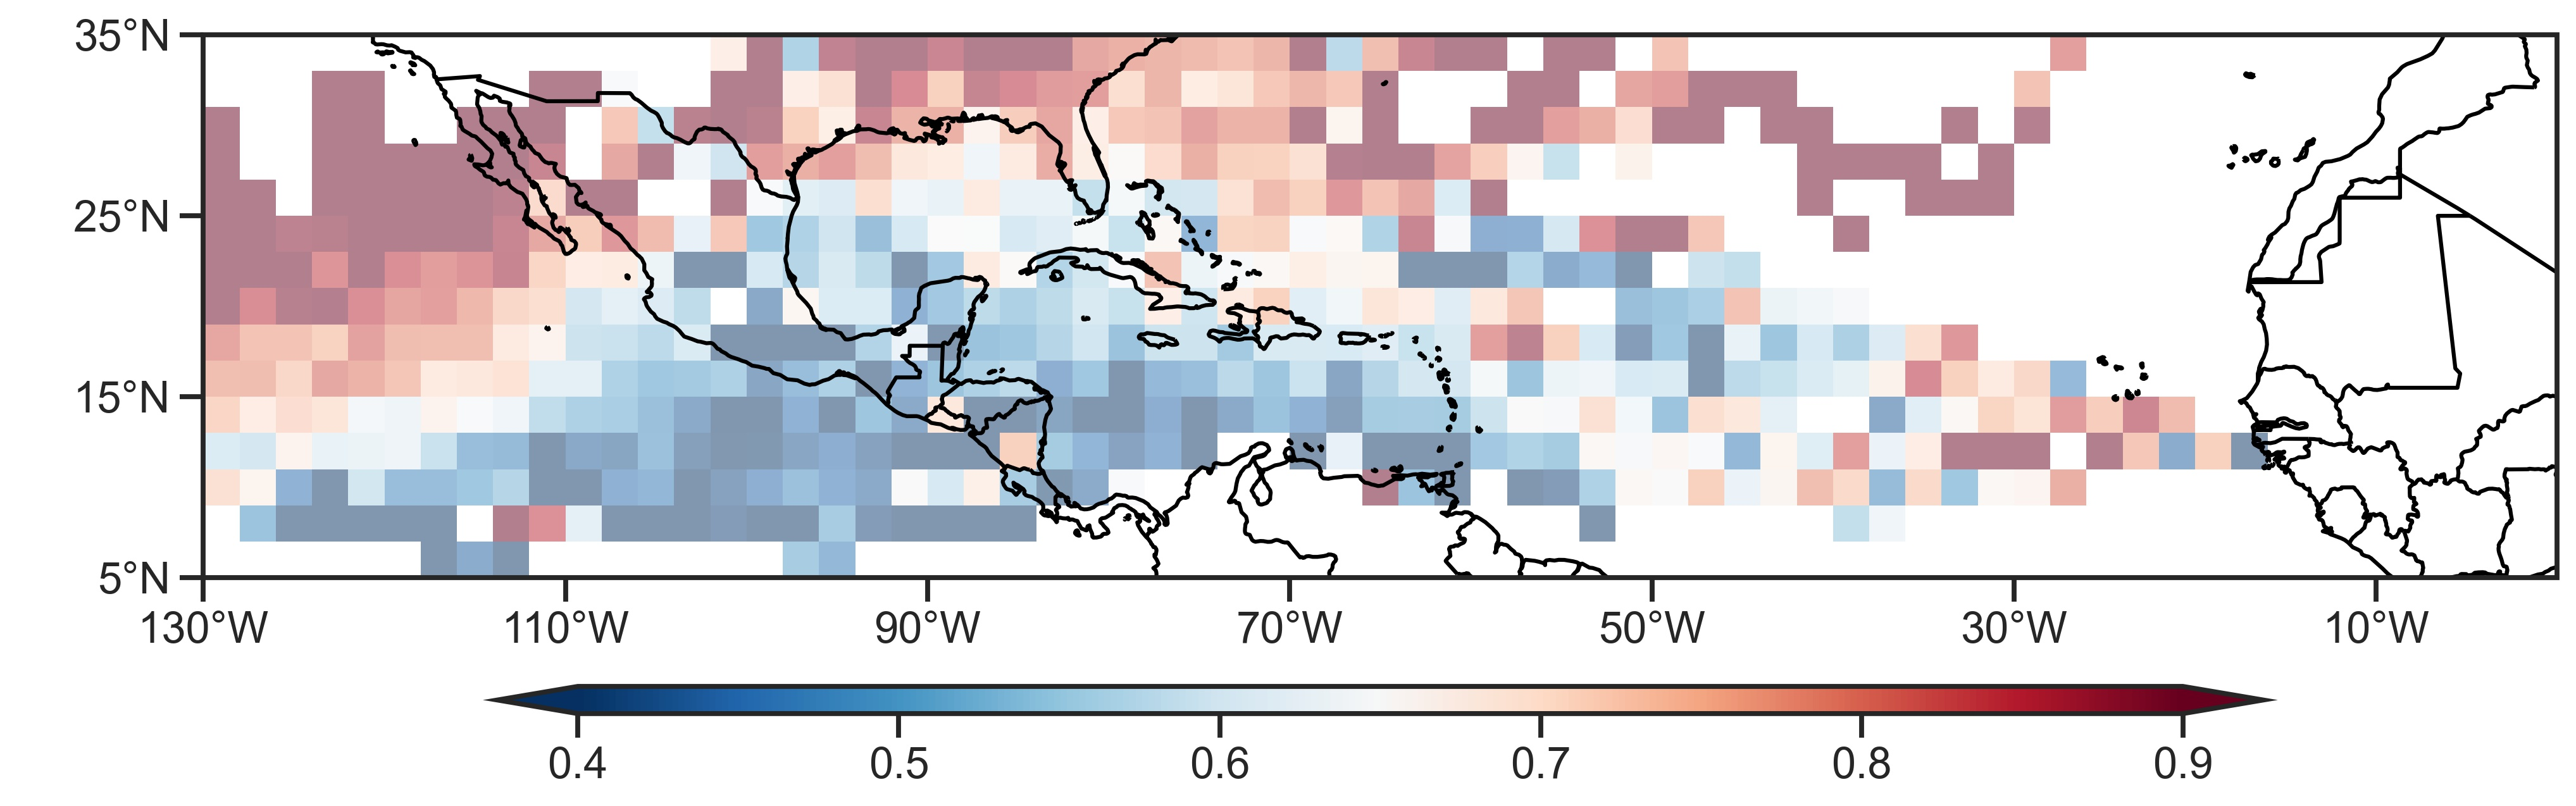
\includegraphics[scale = 0.25]{Images/Figures/Fig_3_27.jpeg}
    \caption{Como en la Fig. \ref{fig:fig_10}, pero para $A$}
    \label{fig:fig_A}
\end{figure}

\begin{figure}
    \centering
    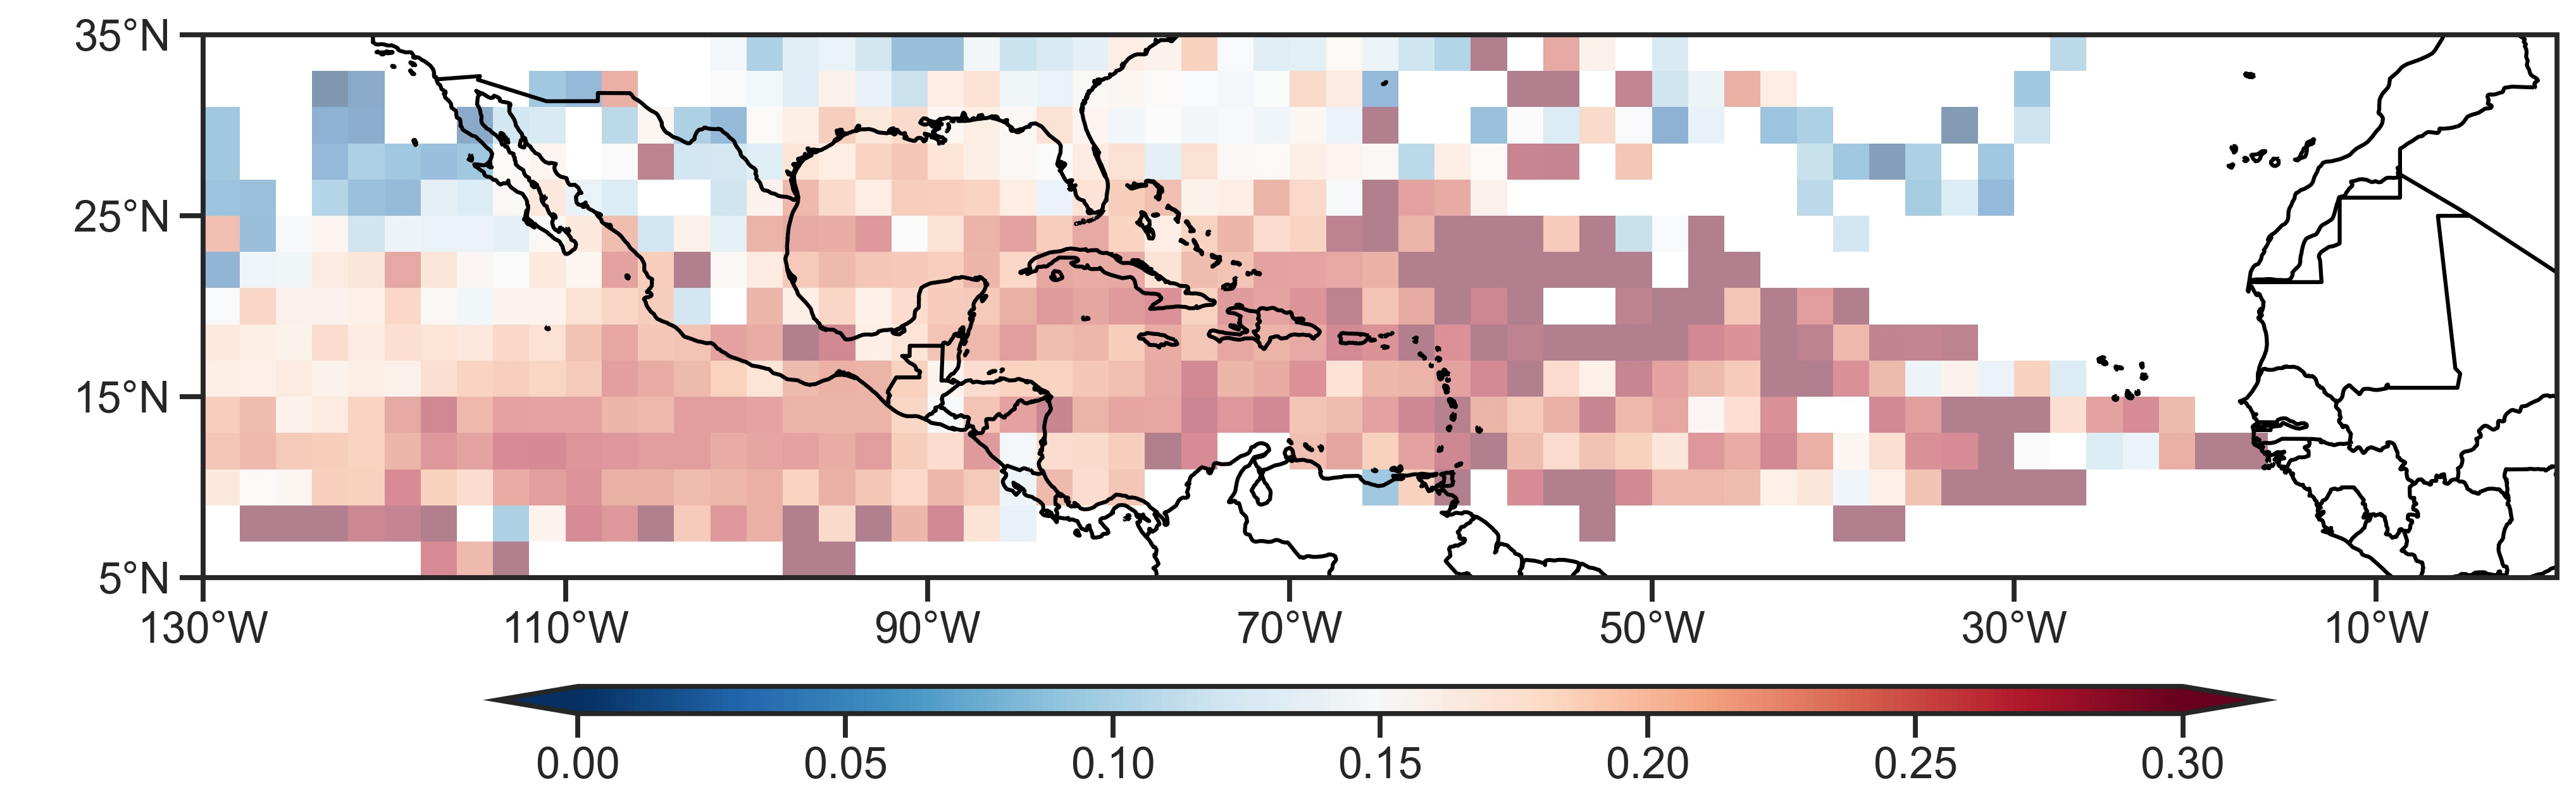
\includegraphics[scale = 0.25]{Images/Figures/Fig_3_28.jpeg}
    \caption{Como en la Fig. \ref{fig:fig_10}, pero para $S$}
    \label{fig:fig_S}
\end{figure}

\end{frame}